\chapter{راهنمای نصب  {\LaTeX}} % شامل \XePersian\  و  \lr{Farsi\TeX}
%\chapter{ثثث}
\section{مقدمه}
نرم‌افزار حروفچینی \TeX یکی از نرم‌افزارهای معروف حروفچینی متون علمی است
که در سطح وسیعی جهت حروفچینی  مجلات و کتب استفاده می‌شود. در این متن مختصر بر آنیم
که راهنمای سریعی برای نصب و استفاده از آن بیان کنیم با این امید که کاربران با پیگیری آن
به راحتی  بتوانند آن را نصب و استفاده نمایند.

قبل از این لازم است جهت واضح شدن شکل عملکرد این نرم افزار، اطلاعاتی در مورد آن داشته
باشیم که در ادامه به آن پرداخته می‌شود.

نرم افزار حروفچینی \TeX یک نرم افزار مجانی است که به صورت خط فرمانی کار می‌کند، به این
معنی که متن مورد نظر در یک فایل نوشته شده و سپس این فایل از طریق دستورات خط
فرمان به نرم افزار حروفچین \TeX داده می‌شود. این نرم افزار فایل داده شده را خوانده و بر
مبنای آن متن حروفچینی شده را به صورت یک فایل (مثلا PDF) ارائه می‌کند.

دستورات خط فرمان متعددی برای استفاده از این نرم افزار حروفچین وجود دارد که از مهمترین 
آنها می‌توان به latex، pdflatex و xelatex اشاره کرد. معمولاً ما این بخش از
نرم افزار حروفچین را موتور \TeX می‌نامیم. این خاصیت، اولین متمایز کنندۀ این نرم‌افزار
از سایر نرم‌افزارها نظیر Office  است زیرا در Office شما نتیجه نهایی را همزمان با تایپ
 می‌بینید ولی در این نرم‌افزار باید فایل را به حروفچین بدهید تا خودش شکل خروجی را آماده
 کند. عملاً به همین دلیل نیز آن را نرم‌افزار حروفچین می‌نامند، مشابه این که شما متن خام 
 خود را به یک فرد حروفچین می‌دهید تا با شکل دهی آن در قالب صفحات، آن را برای چاپ
 آماده کند.
 
 پس متن خام باید در یک ویرایشگر تایپ شده و سپس فایل حاصل (که پسوند آن .tex است)
 به برنامۀ حروفچین
 با استفاده از خط فرمان داده شود. ویرایشگرهایی وجود دارند که امکان وارد کردن متن خام
 و به طور همزمان، امکان دادن فایل به موتور \TeX و نشان دادن نتیجۀ حروفچینی را دارند. 
 اما تمام آنها بر مبنای همان دستورات خط فرمان عمل می‌کنند و هیچکدام به تنهایی و بدون
 دسترسی به یک موتور \TeX نمی‌توانند خروجی تولید کنند. البته هیچ وابستگی بین
 ویرایشگر و فایل تولید شده توسط آن وجود ندارد و یک فایل توسط هر کدام می‌تواند 
 تولید یا ویرایش شود یا فایل ایجاد شده توسط  یک ویرایشگر، در دیگری تغییر یابد.
 از معروف‌ترین این ویرایشگرها می‌توان به WinEdit، Texmaker
و  Notepad++  اشاره کرد.

برای حروفچینی فایل، می‌توان از طریق خط فرمان به صورت زیر عمل کرد. در ویندوز
وارد \lr{Command Prompt } شوید و به محل قرار گرفتن فایل مربوطه (همان فایل با پیوند
.tex) بروید. بسته به کاربرد خود  و شکل خروجی مورد نظر 
یکی از دستورات زیر را بزنید تا فایل خروجی مربوطه ایجاد شود. به جای filename  نام
فایل .tex گذاشته شود. 


\begin{center}
\begin{tabular}{|c|c|}
\hline
برای خروجی .dvi با فایل ورودی انگلیسی & \lr{latex filename}\\  \hline
برای خروجی .pdf با فایل ورودی انگلیسی & \lr{pdflatex filename}\\ \hline
برای خروجی .pdf با فایل ورودی فارسی یا  انگلیسی & \lr{xelatex filename}\\ \hline
\end{tabular}
\end{center}

\textcolor{red}{توجه:} دقت کنید که نام فایل یا فولدرهایی که فایل در آن قرار دارد فارسی
نباشد یا بین نام آنها فاصله وجود نداشته باشد. در صورت عدم رعایت این موضوع، در برخی
مواقع اجرا با مشکل روبرو می‌شود.

فایل آماده شده خام، شامل دستوراتی است که قسمتهای مختلف متن نظیر عنوان فصل و بخش
و سایر موارد را مشخص می‌کند. اگر این دستورات درست استفاده نشده باشند، حروفچین در زمان
حروفچینی خطا می‌دهد که پیام خطا شامل شماره خطی است که در آن خطا اتفاق افتاده است.
لذا، در این موارد باید مشابه خطاگیری از یک برنامۀ کامپیوتری، نسبت به رفع خطا اقدام کرد.
توجه کنید که وجود خطا ممکن است متن را به صورتی به غیر از آنچه مورد نظر است حروفچینی
کند و اگر تعداد خطاها زیاد باشد ممکن است قسمت یا کل متن را حروفچینی نکند و خروجی
نداشته باشد یا خروجی حاصل ناقص باشد.
 
\section{نصب موتور اصلی \TeX}\footnote{فایل‌های مورد استفاده علاوه بر آدرس‌های ذکر شده در اف تی پی دانشگاه یزد به آدرس  
%\begin{verbatim}
\href{ftp://ftp.yazd.ac.ir:8621/Mathematic/TeX}{\lr{ftp://ftp.yazd.ac.ir:8621/Mathematic/TeX}}
%\end{verbatim}
نیز وجود دارد. کاربران متصل به شبکه دانشگاه یزد می‌توانند بدون  نیاز به اتصال به اکانتینگ، این فایل‌ها را با سرعت بالا دانلود نمایند.}
توزیع‌های مختلفی برای موتور \TeX وجود دارد که در اینجا به نصب دو توزیع
معروف و مجانی آن به نام‌های TeXLive  و MikTeX می‌پردازیم. تاکید می‌شود که این توزیع‌ها با هم سازگار هستند، به این
معنی که فایل آماده شده روی تمام توزیع‌های موتور \TeX \ کار می‌کند. لذا مهم نیست کدام
توزیع را برای نصب انتخاب کنید. با نصب هر کدام از این دو توزیع، به طور اتوماتیک
بسته \XePersian \  نصب می‌شود و نیاز به هیچ کار اضافی نیست. فقط لازم است
که فونت‌های فارسی استفاده شده در متون فارسی روی سیستم عامل نصب شده باشد. لذا
تنها کار اضافی این است که مجموعه فونت‌های جمع آوری شده در فایل زیر روی سیستم عامل
نصب شود. توصیه می‌شود حتی اگر فونت‌ها را روی کامپیوتر خود دارید، دوباره آنها را با استفاده
از فونت‌های فایل زیر رونویسی کنید. این کار از بسیاری مشکلات بعدی جلوگیری می‌کند.
\begin{latin}

\href{http://bayanbox.ir/id/4609192605141061595}{Part 1: http://bayanbox.ir/id/4609192605141061595}

\href{http://bayanbox.ir/id/5468937351173971771}{Part 2: http://bayanbox.ir/id/5468937351173971771}

\href{http://bayanbox.ir/id/4133277893427051503}{Part 3: http://bayanbox.ir/id/4133277893427051503}
\end{latin}

البته توصیه پدیدآورندگان بسته \XePersian \ که جهت تولید متون فارسی در \TeX \ 
این بسته را ارائه کرده‌اند، استفاده از  TeXLive  است. 
%\pagebreak
\subsection{نصب \lr{TeXLive 2015}}
%\footnote{با توجه به ارائه نسخه 2015 از TeXLive، این
%نسخه از طریق وبسایت اعلام شده در این قسمت وجود دارد. اما فعلاً این نگارش مشکلاتی با \XePersian دارد. و لذا  نسخه 2014 این نرم افزار را که در اف تی پی دانشگاه یزد وجود دارد دانلود و نصب نمایید. 
%مشکل
%را در \href{http://qa.parsilatex.com/7838/%D9%85%D8%B4%DA%A9%D9%84%D8%A7%D8%AA-texlive-2015-%D9%88-%D8%A7%D8%B1%D8%AA%D9%82%D8%A7-%D8%A8%D8%B3%D8%AA%D9%87-%D9%87%D8%A7-%D8%AF%D8%B1-texlive-2014?show=7838#q7838}{این لینک} ببینید.
%}
سایت‌های معروف به CTAN، سایت‌هایی هستند که  وظیفه توزیع نسخه‌های مختلف
مجانی موتور \TeX را انجام می‌دهند. یکی از این وبسایت‌ها در  دانشگاه یزد 
قرار دارد که در آدرس زیر در دسترس است.\footnote{این وبسایت به همت آقای
مهندس فاطمی از مرکز اطلاع‌رسانی و خدمات رایانه‌ای دانشگاه یزد ایجاد شده است که
جا دارد از ایشان در این خصوص تشکر کرد.}

\centerline{\href{http://ctan.yazd.ac.ir/}{http://ctan.yazd.ac.ir/}}

این سایت به صورت روزانه به روز رسانی می‌شود. می‌توان از این سایت در هر 
لحظه آخرین نگارش‌های نرم افزارهای مربوطه را دانلود کرد. لازم به ذکر است که در صورت اتصال
به شبکه دانشگاه یزد، برای دسترسی به این سایت نیازی به استفاده از اکانتینگ و 
اتصال به اینترنت نیست، بلکه این سایت از طریق شبکه داخلی دانشگاه در دسترس است.

برای نصب TeXLive  مراحل زیر را انجام دهید:
\begin{enumerate}
\item وارد سایت \href{http://ctan.yazd.ac.ir/}{http://ctan.yazd.ac.ir/}
 شوید و در پایین صفحه روی \lr{TeX Live}
 کلیک کنید.
 \item روی مسیر Images کلیک کنید و از فولدر باز شده فایل با نام 
 	\lr{texlive2015-20150523.iso} را دانلود کنید. دقت کنید که 8 شماره آخر فایل ممکن 
	است مختلف باشد زیرا نشان‌دهنده تاریخ ایجاد فایل است. دقت کنید که حجم این فایل
	حدود \lr{2.7} گیگا بایت است.
 \item پس از دانلود کامل، آن را با نرم افزار WinRaR  باز کنید و در  پوشه‌ای به نام
 \lr{TeXLive2015} فایل را Extract کنید.
 \item وارد این پوشه شوید و برنامه 
 %install-tl
\lr{install-tl-windows}
 را اجرا کنید. ادامه روند مشابه نصب سایر نرم افزارها 
 است. روند نصب بسته به سرعت کامپیوتر شما ممکن است تا 1 ساعت طول بکشد.
 تصویر پنجره‌های نصب به صورت زیر است (به ترتیب از چپ به راست و از بالا به پایین)
\latin
\begin{figure}[htb]
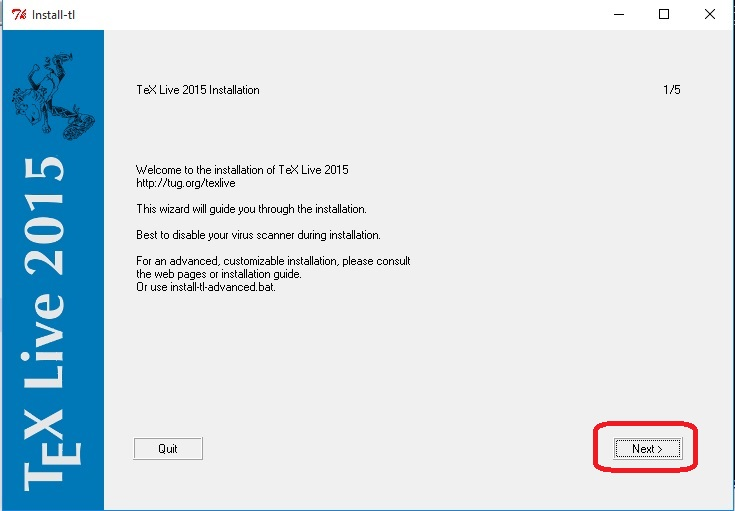
\includegraphics[width=0.45\textwidth]{TexLive2015-1}\hfill
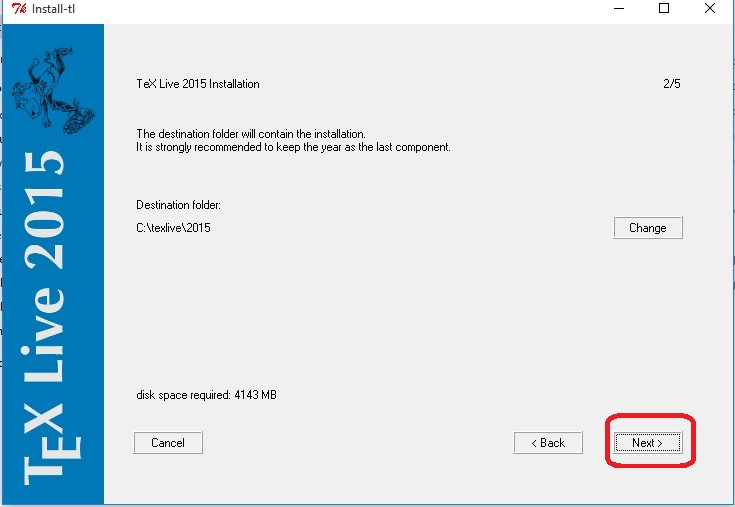
\includegraphics[width=0.45\textwidth]{TexLive2015-2}
\vspace*{4mm}

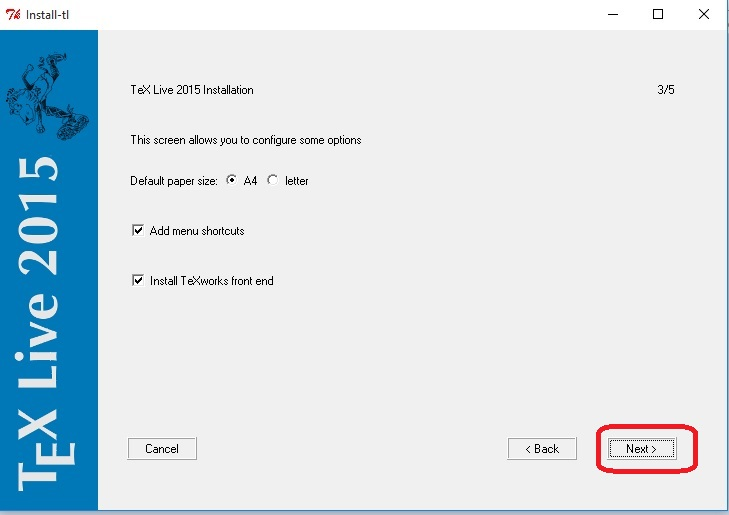
\includegraphics[width=0.45\textwidth]{TexLive2015-3}\hfill
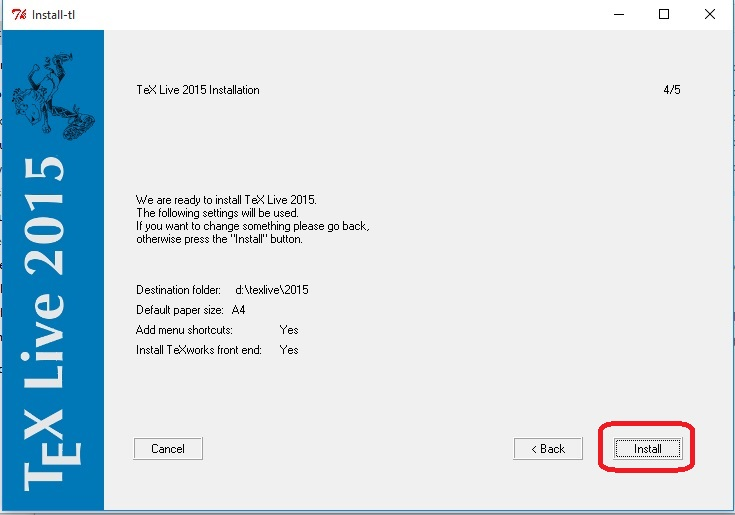
\includegraphics[width=0.45\textwidth]{TexLive2015-4}
\vspace*{4mm}

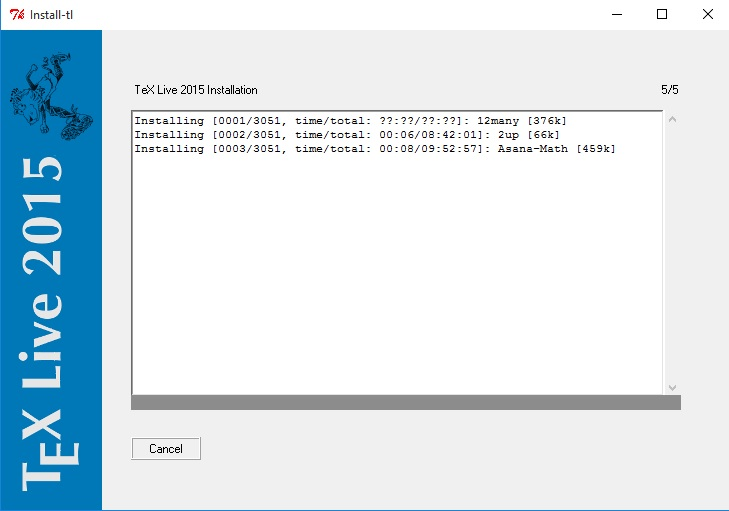
\includegraphics[width=0.45\textwidth]{TexLive2015-5}\hfill
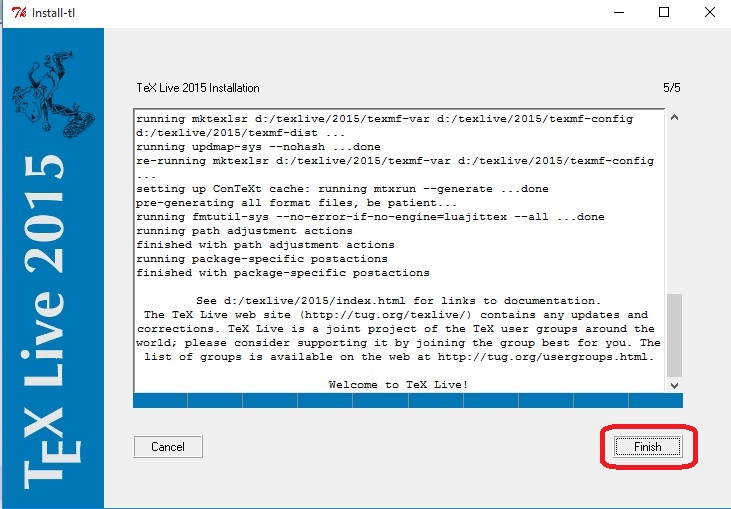
\includegraphics[width=0.45\textwidth]{TexLive2015-6}
\vspace*{4mm}
%
%\includegraphics[width=0.45\textwidth]{install-6}
\persian
\caption{پنجره‌های نصب \lr{TeXLive 2015} (ترتیب از چپ به راست)}
\end{figure}
\persian

 \item پس از پایان نصب، موتور \TeX آماده استفاده است. اگر قصد استفاده از \XePersian
 \ دارید، فقط لازم است فونت‌های مربوطه را که در بالا لینک آن آمده است را نصب کنید.
\end{enumerate}
بهتر است بعد از نصب؛ بسته های این نرم افزار را با روش زیر به روز رسانی کنید.
\subsubsection{بروزرسانی بسته‌های \lr{TeXLive 2015}}
دقت کنید که برای بروزرسانی شما باید به اینترنت متصل باشید زیرا بروزرسانی با استفاده از اینترنت انجام می‌شود.
\begin{enumerate}
\item ابتدا در قسمت برنامه‌ها، برنامه \lr{TeX Live manager} را اجرا کنید.
\item مطابق شکل زیر، مسیر به روزرسانی را \url{ctan.yazd.ac.ir} انتخاب کنید. انتخاب هر مسیر دیگر اشکالی ندارد ولی روی سرعت گرفتن فایل‌ها تاثیر دارد. 
\item ابتدا مطابق شکل، بسته مشخص شده را به روزرسانی کنید. پس از بروز رسانی این بسته، برنامه بسته می‌شود و لازم است دو مرحله قبل را دوباره تکرار کنید.
\item حال روی \lr{Updtate all installed} کلیک کنید. به روزرسانی نیز مشابه نصب مدت زمانی که به سرعت کامپیوتر و سرعت اینترنت شما وابسته است طول می‌کشد.
\end{enumerate}
%\endinput
\latin
\begin{figure}[h]
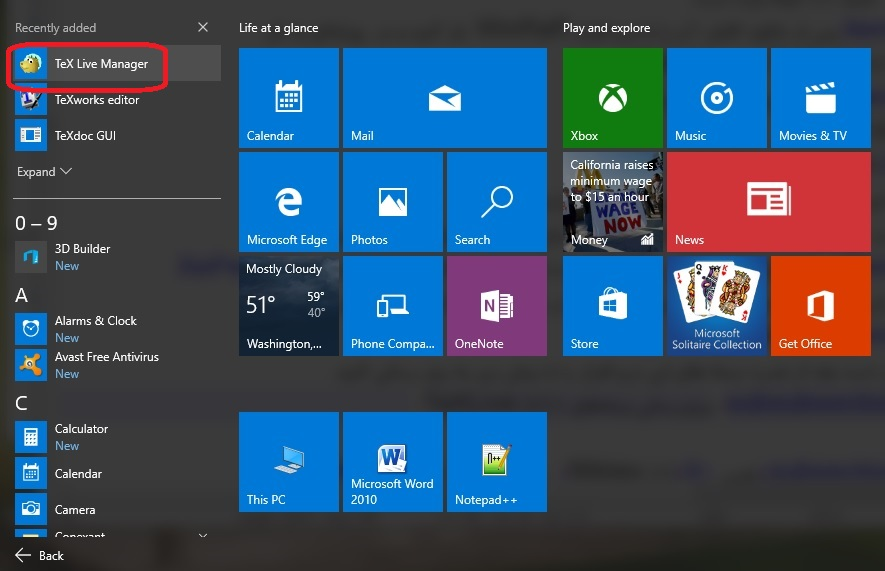
\includegraphics[width=0.4\textwidth]{TexLive2015-Update-1}\hfill
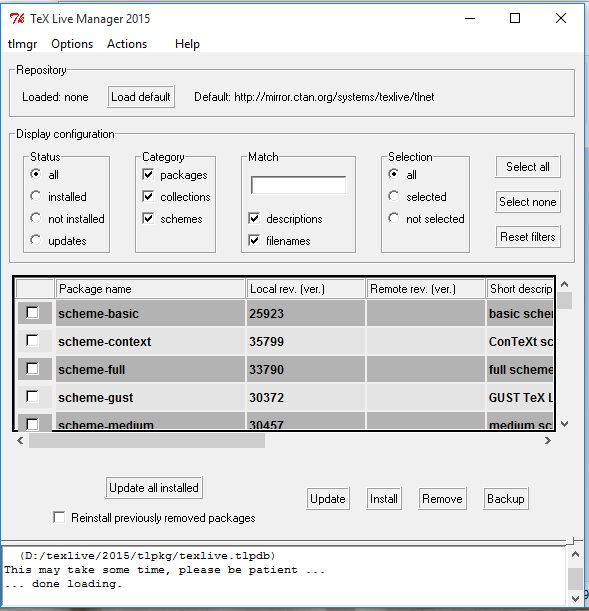
\includegraphics[width=0.4\textwidth]{TexLive2015-Update-2}
\vspace*{4mm}

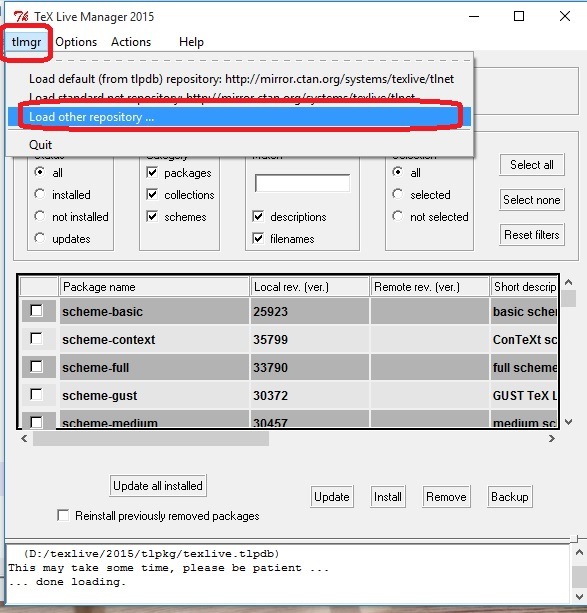
\includegraphics[width=0.4\textwidth]{TexLive2015-Update-3}\hfill
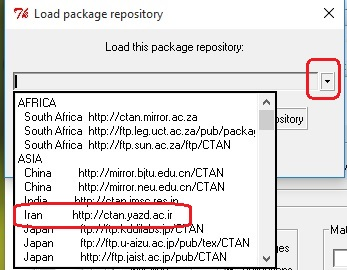
\includegraphics[width=0.4\textwidth]{TexLive2015-Update-4}
\vspace*{4mm}

%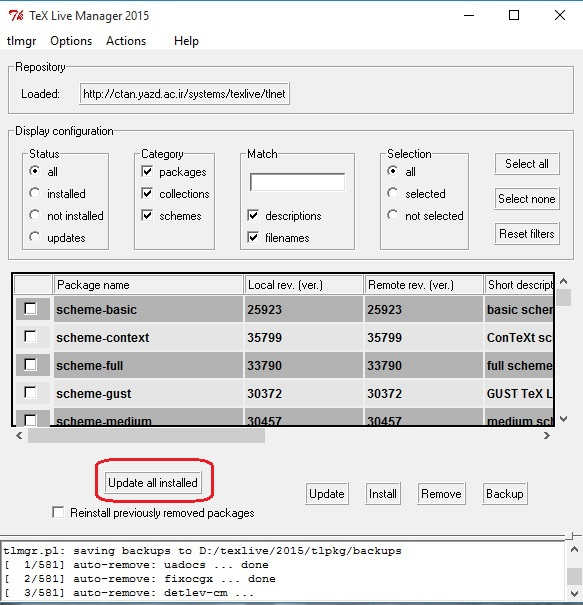
\includegraphics[width=0.4\textwidth]{TexLive2015-Update-5}\hfill
%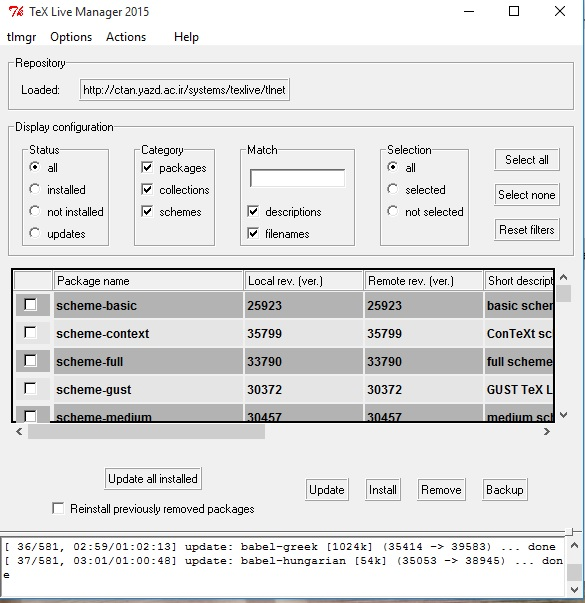
\includegraphics[width=0.4\textwidth]{TexLive2015-Update-6}
%\vspace*{4mm}

%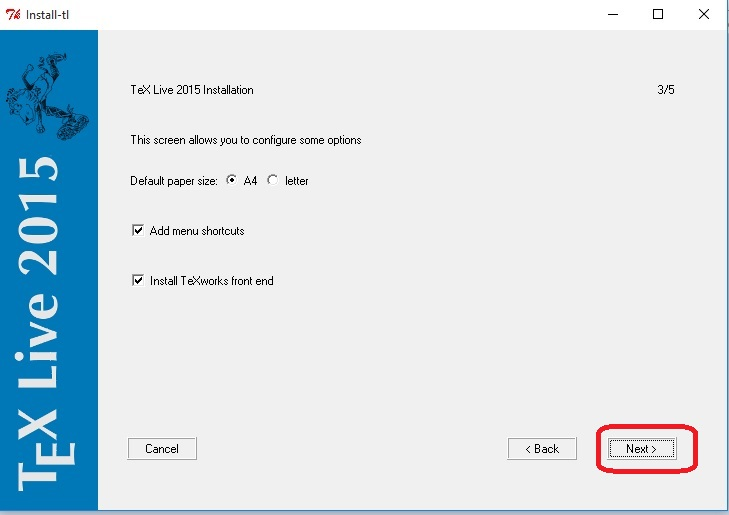
\includegraphics[width=0.45\textwidth]{TexLive2015-3}\hfill
%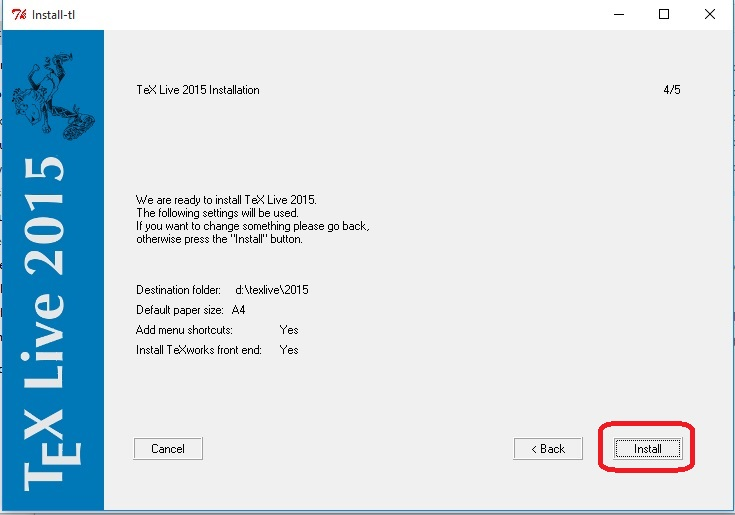
\includegraphics[width=0.45\textwidth]{TexLive2015-4}
%\vspace*{4mm}

%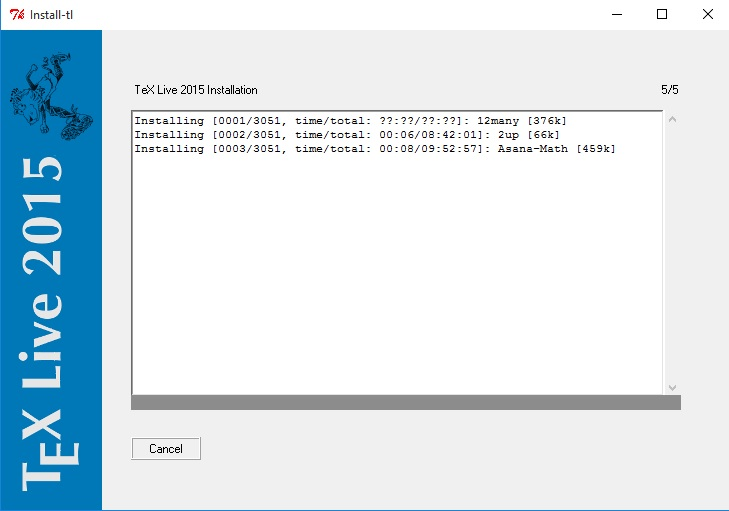
\includegraphics[width=0.45\textwidth]{TexLive2015-5}\hfill
%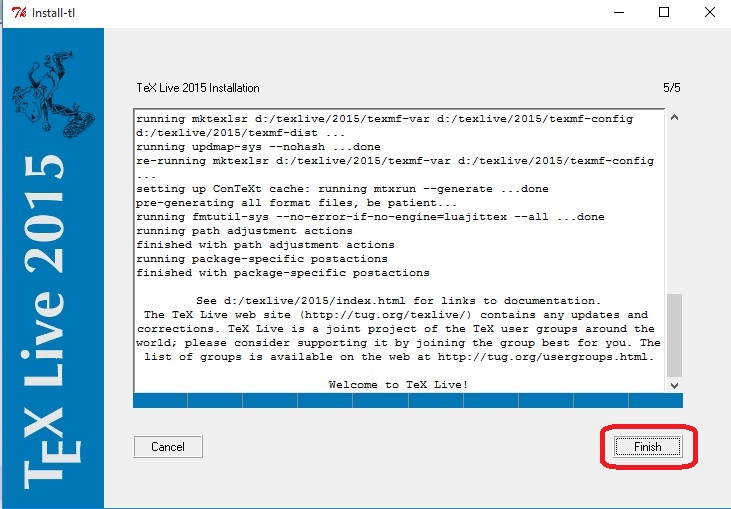
\includegraphics[width=0.45\textwidth]{TexLive2015-6}
%\vspace*{4mm}
%
%\includegraphics[width=0.45\textwidth]{install-6}
\persian
\caption{پنجره‌های بروزرسانی \lr{TeXLive 2015} (ترتیب از چپ به راست)}
\end{figure}
\begin{figure}[t]
%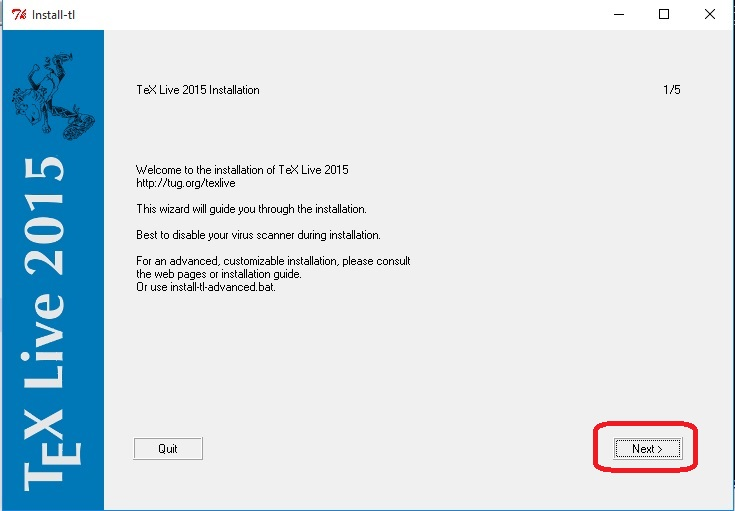
\includegraphics[width=0.45\textwidth]{TexLive2015-1}\hfill
%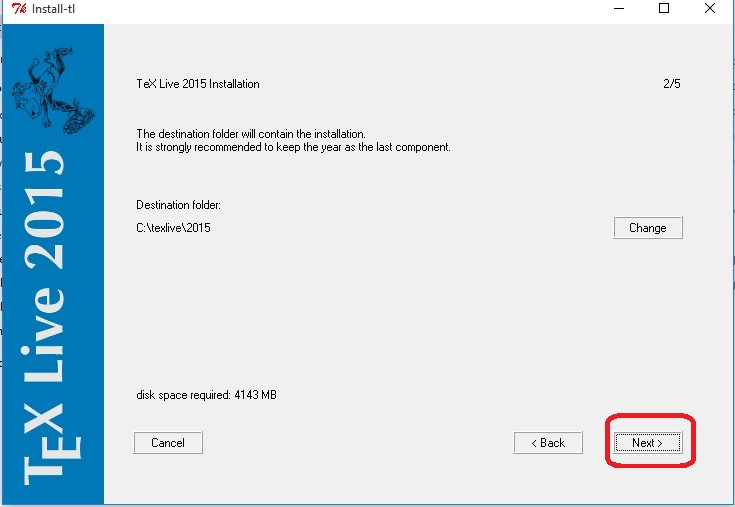
\includegraphics[width=0.45\textwidth]{TexLive2015-2}
%\vspace*{4mm}
%

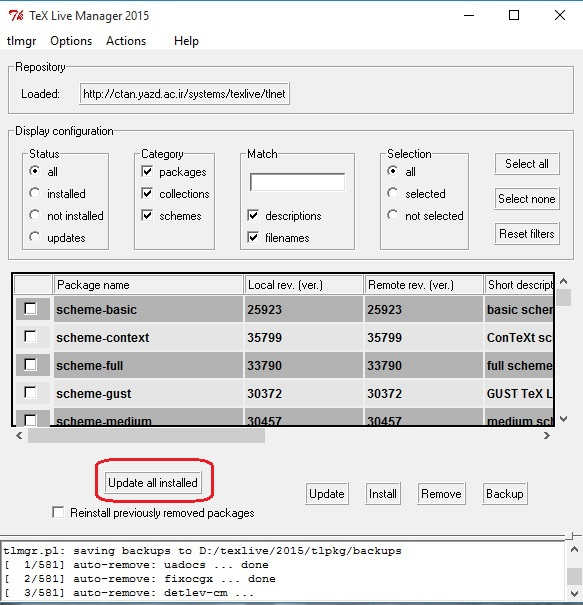
\includegraphics[width=0.4\textwidth]{TexLive2015-Update-5}\hfill
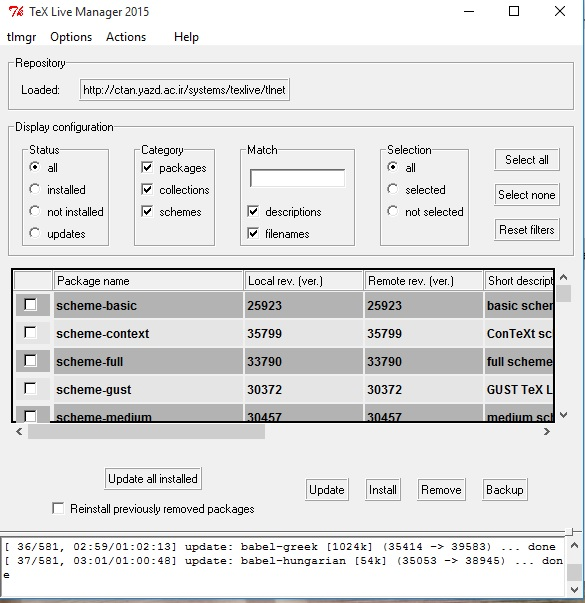
\includegraphics[width=0.4\textwidth]{TexLive2015-Update-6}
\vspace*{4mm}

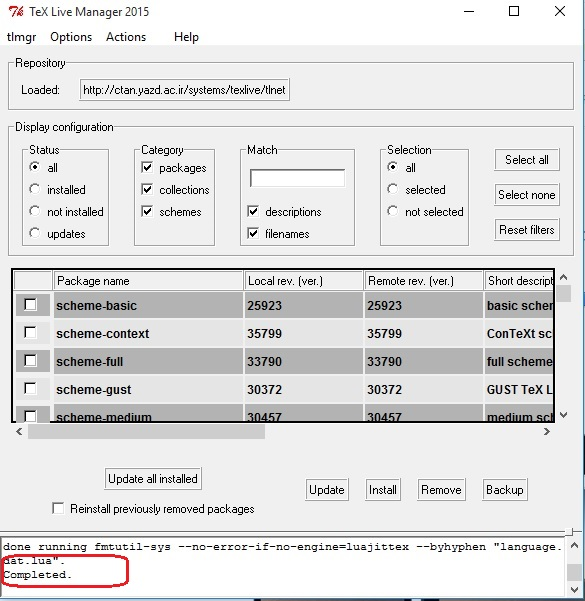
\includegraphics[width=0.45\textwidth]{TexLive2015-Update-7}
\persian
\caption{ادامه پنجره‌های بروزرسانی  \lr{TeXLive 2015}  (ترتیب از چپ به راست)}
\end{figure}

\persian
\newpage 
\pagebreak
\subsection{نصب  \lr{Miktex 2.9}   به طور کامل (\XePersian)}
\baselineskip=1cm
\begin{enumerate}
\item برای دانلود فایل‌های لازم از یکی از روش‌های زیر استفاده کنید:
\begin{itemize}
\item اگر به شبکه دانشگاه یزد دسترسی دارید (به شبکه داخلی دانشگاه متصل هستید) بدون نیاز به اتصال
به اکانتینگ، از لینک زیر فایل مربوطه را دانلود کنید:

\centerline{\lr{ftp://ftp.yazd.ac.ir:8621/Mathematic/TeX/}}

توجه کنید که این فایل لزوماً آخرین نگارش نرم افزار نیست ولی برای اجرا مشکلی ندارد. پس از دانلود
فایل فشرده را باز کنید.

\item دانلود فایل \lr{setup-2.9.4503.exe} از مسیر زیر و اجرای آن و انتخاب گزینۀ دانلود برای دانلود فایل‌های لازم.

\lr{http://ctan.yazd.ac.ir/systems/win32/miktex/setup/}

دقت کنید که شماره پایانی ممکن است در نگارش‌های جدیدتر متفاوت باشد.
این نرم افزار تمام فایل‌های لازم را دانلود و در مسیری که مشخص کرده‌اید ذخیره می‌کند.
برای انتخاب محل از \lr{ctan.yazd.ac.ir} استفاده کنید.
\item دانلود تمام بسته‌ها مستقیماً از مسیر زیر:\\
\lr{http://ctan.yazd.ac.ir/systems/win32/miktex/tm/packages/}
\end{itemize}
\item   از پوشه مربوطه، فایل \lr{setup-2.9.4503.exe}  را اجرا کنید.  (شکل 1 را ببینید\footnote{شکل‌ها مربوط
به \lr{MikTeX2.8} است ولی مشابه شکل‌های اجرا است. }).
\item در پنجرۀ باز شده \lr{Accept the Miktex ...} را تیک زده و روی \lr{Next} کلیک کنید.
\item \label{complete} در پنجره بعدی \lr{Complete Miktex} را انتخاب کنید و روی \lr{Next} کلیک کنید.

\item  در پنجره بعدی \lr{Anyone who use ...}  را انتخاب کنید و روی \lr{Next} کلیک کنید.
\item  در پنجره بعدی  مسیر مورد نظر برای نصب را انتخاب کنید و روی \lr{Next} کلیک کنید. دقت کنید که تمام نام مسیر باید به 
انگلیسی باشد وگرنه در اجرای برنامه مشکل ایجاد خواهد شد. نصب برنامه به فضای هارد تقریبا 2 گیگا بایت نیاز دارد و روند نصب
بسته به سرعت کامپیوتر شما ممکن است تا 2 ساعت طول بکشد.
\item  پس از اتمام نصب، فونت‌های موجود در پوشه \lr{Xepersian-fonts} را روی ویندوز نصب نمایید.
توصیه می‌شود در صورت موجود بودن فونت‌ها، آنها رونویسی شوند.
\item در این مرحله \XePersian نصب شده و قابل استفاده است.
\item  جهت ویرایش متون خود باید از ادیتورهای پشتیبانی کننده یونیکد استفاده نمایید. نوع ادیتور نقشی در فرآیند حروفچینی ندارد. در ادامه
نصب و استفاده از \lr{Notepad++ } آمده است.
\end{enumerate}
\latin
\begin{figure}
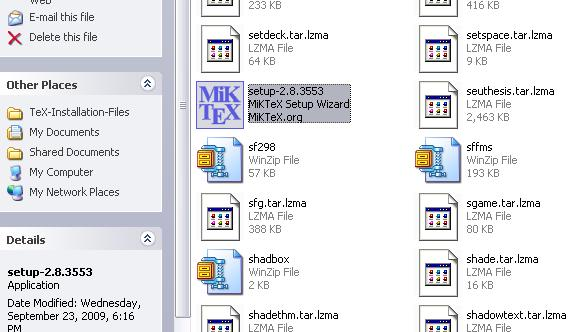
\includegraphics[width=0.45\textwidth]{Setup}\hfill
\includegraphics[width=0.45\textwidth]{install-1}
\vspace*{4mm}

\includegraphics[width=0.45\textwidth]{install-2}\hfill
\includegraphics[width=0.45\textwidth]{install-3}
\vspace*{4mm}

\includegraphics[width=0.45\textwidth]{install-4}\hfill
\includegraphics[width=0.45\textwidth]{install-5}
\vspace*{4mm}

\includegraphics[width=0.45\textwidth]{install-6}
\persian
\caption{پنجره‌های نصب \lr{MikTeX 2.9} (ترتیب از چپ به راست)}
\end{figure}
\persian
\section{ناسازگاری فایل‌های قبلی آماده شده با زیپرشن }
پس از نصب \lr{MikTeX2.9} با اجرای فایل‌های قبلی ممکن است با پیغام خطای زیر مواجه شوید:
\latin
\begin{verbatim}
! Undefined control sequence.
\SetMathCode #1#2#3#4->\Umathcode 
                       #1="\mathchar@type #2 \csname sym#3\endcsn...
\end{verbatim}
\persian
برای رفع خطا دستورات زیر را در خط بعد از دستور $\backslash$ documentclass بگذارید:
\latin
\begin{verbatim}
\makeatletter
\@ifundefined{Umathcode}{\let\Umathcode\XeTeXmathcode}{}
\@ifundefined{Umathchardef}{\let\Umathchardef\XeTeXmathchardef}{}
\makeatother 
\end{verbatim}
\persian
\section{نصب Notepad++}
\baselineskip=1cm
ادیتور \lr{Notepad++ }  به دلیل قابلیت فارسی نویسی و همچنین از راست به چپ نویسی و امکان اجرای دستورات خط فرمان در ادیتور،
انتخاب مناسبی برای نوشتن متون  است. برای فعال کردن قابلیت اجرای دستورات خط فرمان با استفاده از کلید \lr{F6}، پس از نصب نرم افزار
\lr{Notepad++ }، فایل \lr{NppExec\_030\_dll\_Unicode.zip}
را در پوشه plugins  از مسیری که \lr{Notepad++ }  در آن نصب شده است باز کنید. حال با زدن کلید \lr{F6}  در ادیتور، پنجره اجرای دستور باز می‌شود.

نمونه دستوری که می‌توانید وارد کنید به صورت زیر است:

\begin{latin}
\begin{verbatim}
NPP_SAVE
cd $(CURRENT_DIRECTORY)
xelatex $(NAME_PART)
\end{verbatim}
\end{latin}

برای تایپ از راست به چپ کلیدهای \lr{Alt+CTRL+R}  را بزنید و برای از چپ به راست نویسی کلیدهای \lr{Alt+Ctrl+L}  را بزنید.

برای نیم فاصله، کلید استاندارد \lr{Ctrl+SHift+2}  است که در این ادیتور به دلیل استفاده از این ترکیب برای کار دیگری عمل نمی‌کند.
برای عمل کردن آن باید این ترکیب کلید را از ادیتور حذف کنید. برای این منظور از منوی \lr{settings -> Shortcut Mapper}
 در برگه \lr{Main Menu}  در ردیف حدودا 80  این ترکیب را پیدا کرده و به چیز دیگری (مثلا \lr{CTRL+Shift+T}) عوض کنید.

 پس از این کار ترکیب  \lr{Ctrl+SHift+2} برای نیم فاصله (وقتی زبان فارسی باشد) کار می‌کند.
 
 توجه: برای تهیه فایل مقاله یا کتاب با \XePersian، باید از کد \lr{UTF8}  برای کدگذاری فایل استفاده شود. برای انتخاب در ادیتور، از منوی
 Encoding  گزینه مورد نظر انتخاب شود.
 \section{کلاس پایان‌نامه دانشگاه یزد}
 با توجه به تنظیمات خاص پایان‌نامه‌های دانشگاههای مختلف و وقت قابل ملاحظه‌ای که انجام این تنظیمات از دانشجویان می‌گیرد، کلاسی بر مبنای تنظیمات پایان نامه‌های دانشگاه یزد ایجاد شده است و از طریق وبسایت زیر در دسترس دانشجویان عزیز می‌باشد.
 
 \centerline{\href{http://yazd-thesis.blog.ir/}{http://yazd-thesis.blog.ir/}}
 
 در این کلاس کلیه تنظیمات مربوط به پایان نامه لحاظ شده و نیاز به انجام تنظیمات اضافی ندارد. توضیحات استفاده از این کلاس و فایل نمونه در وبسایت فوق آمده است.
 %\pagebreak
 \section{تبدیل فایل‌های Word  به \LaTeX\   و برعکس}
 یک نرم افزار قوی برای تبدیل بین Word  و \LaTeX، نرم‌افزار \href{http://www.grindeq.com/}{GrindEQ}  است.
 این نرم‌افزار مجانی نیست ولی تا 10 فایل را برای شما تبدیل می‌کند. برای انجام تبدیل لازم است نرم‌افزار \lr{Office 2010}  را نصب و سپس
 دو فایل مربوط به تبدیل بین Word  و \LaTeX  (در پوشه Convert وجود دارد) را نصب نمایید.
 برای نسخه‌های بعدی \lr{Office}، آخرین نگارش نرم‌افزار را از وبسایت فوق دریافت و نصب نمایید. نرم‌افزار منطبق بر آفیس را (از حیث 32 بیتی یا 64 بیتی بودن) را نصب کنید وگرنه عملکرد تبدیل مناسب نخواهد بود.
 \subsection{تبدیل Word به \LaTeX}
 فایل خود را در Word باز کنید. سپس از منوی \lr{File}،
 \lr{Save As}  را انتخاب کنید و در قسمت \lr{Save as Type}، نوع \lr{LaTeX[GrindEQ]}
 را انتخاب کنید.  از پنجره باز شده گزینه‌های مناسب را انتخاب و فایل را ذخیره کنید. فایل ذخیره شده با فرمت \LaTeX \  است.
 
 اگر فایل Word شما \textcolor{red}{\bf فارسی} است، باید از پنجره باز شده، در قسمت encoding، 
 گزینۀ UTF8 یا Unicode  را انتخاب کنید. (شکل 3 را ببینید.) در فایل
 \LaTeX \ ایجاد شده نیز باید دستور \verb+ \usepackage{xepersian}+  و دستورات مربوط به فونت متن اضافه شود.
 
 همچنین در قسمتهای انگلیسی باید دستور \verb+\latin+  قبل از متن انگلیسی و \verb+\persian+ بعد از متن انگلیسی قرار گیرد.
 
 \subsection{تبدیل \LaTeX \ به Word}
  در Word   فایل \LaTeX  را باز کنید (فایل با پسوند \lr{.tex}). از پنجره باز شده مشابه قبلی، گزینه‌های مناسب را انتخاب کنید. فایل  به فرمت 
  Word تبدیل شده و باز می‌شود و می‌توانید آن را ذخیره کنید. امکان انتخاب فونت و سایر خواص در پنجره باز شده هنگام تبدیل ممکن است.
  
  مشابه قبل، اگر فایل \LaTeX \ شما \textcolor{red}{\bf فارسی} است، باید از پنجره باز شده، در قسمت encoding، 
 گزینۀ \lr{UTF8} یا Unicode  را انتخاب کنید. (شکل 3 را ببینید.)  
\latin
\begin{figure}
\begin{center}
\includegraphics[width=0.45\textwidth]{Word2Latex} %\hfill
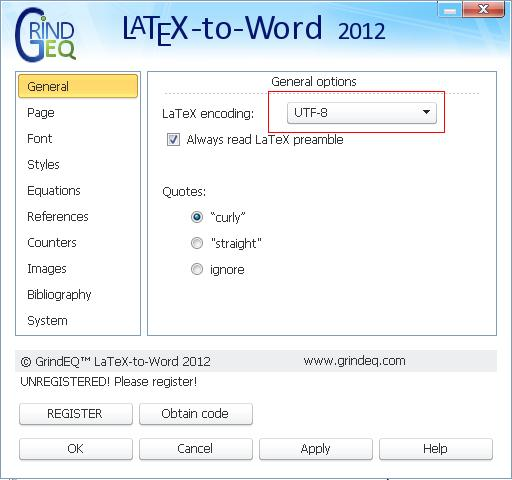
\includegraphics[width=0.45\textwidth]{Latex2Word}
\end{center}
\persian
\caption{پنجره تبدیل Word  به \LaTeX\  (سمت  چپ ) و \LaTeX\  به Word (سمت راست).}
\end{figure}

  \persian 

{\bf توجه:} با توجه به این که امکان تبدیل فایل‌های   \lr{Farsi\TeX} به یونیکد در زیر بیان شده است، می‌توان پس از تبدیل
این فایل‌ها به یونیکد، آنها را با استفاده از ابزار فوق به Word  نیز تبدیل کرد. البته این مورد از نظر کیفیت انجام آزمایش نشده است.
 %\pagebreak 
\section{نصب  \lr{Farsi\TeX}}
\baselineskip=1cm
\begin{enumerate}
\item ابتدا \lr{MikTeX2.9} را نصب کنید.\footnote{امکان نصب فارسی تک روی
TeXLive نیز باید ممکن باشد ولی برای آن فعلا دستورالعملی نیست. می‌توانید دستورات معادل
این دستورات را در TeXLive اجرا کنید تا نتیجه را ببینید. با توجه به به روز رسانی نشدن فارسی تک
و همچنین مشکلات مربوط به ادیتور آن با ویندوزهای جدید و همچنین با توجه به این که فایل‌های
قدیمی نوشته شده در فارسی تک را به راحتی می‌توان به زیپرشن تبدیل کرد، به مقوله 
نصب فارسی تک زیاد پرداخته
نشده است.}
 در ادامه، فرض می‌کنیم این نرم افزار در مسیر 
\lr{C:$\backslash$miktex2.9} 
 نصب شده است.
در صورتی که برنامه در مسیر دیگری نصب شده است مسیر جدید جایگزین مسیر فوق در ادامه روند گردد.
\item فایل  \lr{farsitex-1.0-alpha-3} را در  مسیر \lr{C:$\backslash$miktex2.9}   باز  (unzip)  کنید. 
(فایل‌های این قسمت در پوشه FarsiTeX موجودند).
\item  ادیتور فارسی تک در مسیر \lr{Editor1}   را در مسیر \lr{C:$\backslash$miktex2.9$\backslash$miktex$\backslash$bin} 
نصب کنید. دقت کنید که معمولا bin  آخر توسط برنامه گذاشته می‌شود.
\item  فایل فشرده \lr{ftexed10-840121}  را که در مسیر \lr{Editor2} قرار دارد روی مسیر  \lr{C:$\backslash$miktex2.9$\backslash$miktex$\backslash$bin} 
باز کنید. در اینجا سوال پرسیده می شود که فایل وجود دارد و آیا رونویسی شود که بله را انتخاب کنید.
\item  در قسمت \lr{Start $\Longrightarrow$ Run} دستور \lr{mo$\_$admin} را اجرا کنید.
\item  در پنجره باز شده، روی \lr{Refresh FNDB} کلیک کنید و منتظر بمانید تا کار انجام شود.
\item  در همین پنجره، روی منوی Formats کلیک کنید و روی New کلیک کنید و جدول را مطابق اطلاعات زیر به طور دقیق تکمیل کنید.
در تکمیل دقیق اطلاعات این قسمت دقت کنید وگرنه فارسی تک اجرا نخواهد شد.
\begin{latin}
{\bf Format key:} {\Large farsitex}\\
{\bf Format name:} {\Large farsitex}\\
{\bf Compiler:} {\Large pdftex}\\
{\bf Input file name:} {\Large farsitex.ini}\\
{\bf Output file name:} {\Large farsitex.efmt}\\
{\bf Preloaded Format:} \\
{\bf Description:} {\Large FarsiTeX }\\
\end{latin}
 قسمت مربوط به \lr{Preloaded Format} خالی گذاشته شود. 
\item پس از وارد کردن اطلاعات و زدن OK عبارت FarsiTeX در جدول سمت چپ ظاهر می‌شود. روی آن کلیک کرده
و سپس روی Build کلیک کنید. پس از اتمام کار پنجره را ببندید.
\item  در مسیر 
\lr{C:$\backslash$miktex2.9$\backslash$tex$\backslash$latex209$\backslash$base} 
اسامی فایل‌های \lr{x.sty} را به \lr{x209.sty} (فقط برای فایل‌های article book، و report ) تغییر دهید. به عنوان مثال \lr{article.sty} به \lr{article209.sty} تغییر کند. با این کار
در فایل‌های فارسی‌تک نیز باید به جای \lr{article} در دستور $\backslash$documentstyle به \lr{article209} تبدیل شود.
\item  در قسمت \lr{Start $\Longrightarrow$ Run} دستور \lr{mo$\_$admin} را اجرا کنید. (بله! تکراری است ولی باید تکرار شود.)
\item  در پنجره باز شده، روی \lr{Refresh FNDB} کلیک کنید و منتظر بمانید تا کار انجام شود.
\item  در صورت تمایل به نصب فونت لوتوس، فایل lotusfont.zip  را در مسیر  \lr{C:$\backslash$miltex2.9}
باز کنید و سپس در قسمت  \lr{Start $\Longrightarrow$ Run} دستور \lr{initexmf\ \    -u} را اجرا کنید.
\item  در قسمت \lr{Start $\Longrightarrow$ Run} دستور \lr{mo$\_$admin} را اجرا کنید. (بله! تکراری است ولی باید تکرار شود.)
\item  در پنجره باز شده، روی \lr{Refresh FNDB} کلیک کنید و منتظر بمانید تا کار انجام شود.

%\item  جهت ویرایش متون خود باید از ادیتورهای پشتیبانی کننده یونیکد استفاده نمایید. نوع ادیتور نقشی در فرآیند حروفچینی ندارد.
%\item  جهت ویرایش متون خود باید از ادیتورهای پشتیبانی کننده یونیکد استفاده نمایید. نوع ادیتور نقشی در فرآیند حروفچینی ندارد.
\end{enumerate}
\section{تبدیل فایل های فارسی تک به زیپرشن}

نرم‌افزار تبدیل فایل‌های فارسی تک به زیپرشن توسط آقای دکتر واحدی آماده شده است. این نرم‌افزار با زبان Python نوشته
شده و برای اجرا لازم است آن را روی کامپیوتر نصب نمایید. جزئیات اجرا از راهنمای زیپرشن در زیر آمده است.
\begin{center}
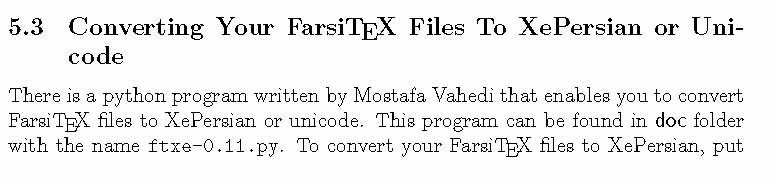
\includegraphics[width=\textwidth]{farsitex2xepersian-1.jpg} 
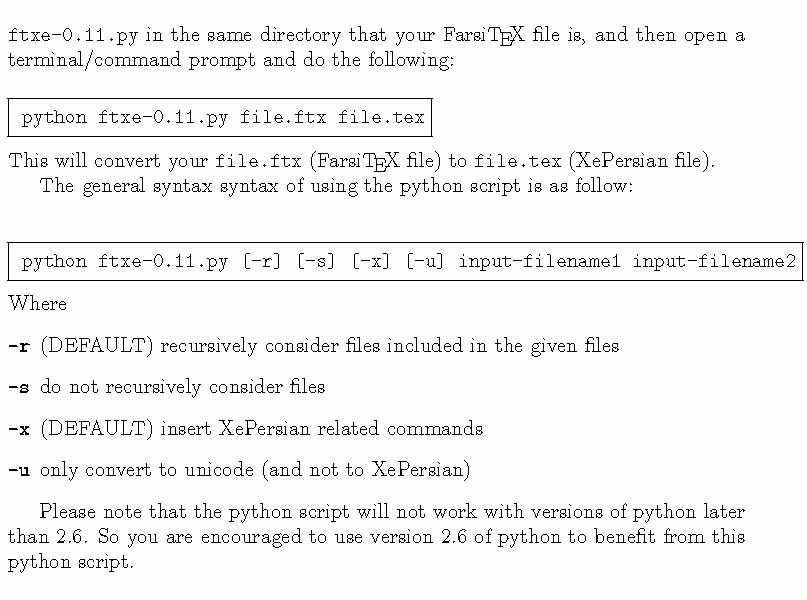
\includegraphics[width=\textwidth]{farsitex2xepersian-2.jpg} 
%
\includegraphics[width=\textwidth]{farsitex2xepersian-p1} 
%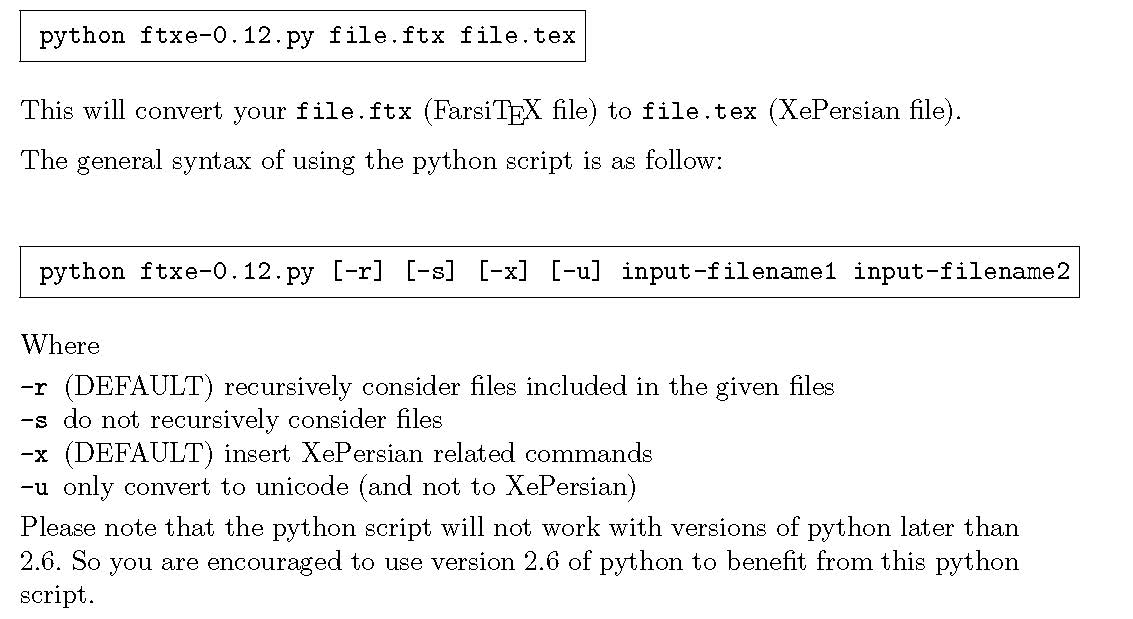
\includegraphics[width=\textwidth]{farsitex2xepersian-p2} 
\end{center}

انتخاب دیگر برای تبدیل، بازکردن فایل با استفاده از \lr{bidi-TeXMaker} است. این نرم افزار دارای منوی \lr{Import FTX File(s)} در منوی \lr{File} است. با باز کردن فایل‌های با پسوند \lr{.FTX}، فایل تبدیل  به یونیکد می‌شود.
\section{جزئیات فارسی نویسی در \lr{IPE Drawing}}
نرم‌افزار مجانی \lr{Ipe Drawing} که یک ابزار قوی برای رسم اشکال است و بر مبنای \TeX\ کار می‌کند 
نسخه جدید خود را منتشر کرد. این نسخه شامل فایل باینری برای سیستم‌های ویندوزی نیز هست. این نگارش 
جدید را علاوه بر وبسایت آن به آدرس \url{http://ipe.otfried.org/}
  می‌توانید از لینک زیر نیز دریافت کنید. این ابزار امکان درج فرمول‌های ریاضی و متون فارسی و همچنین درج تصاویر 
  با فرمت‌های bmp  و jpg  را نیز می‌دهد. لازم به ذکر است که برای اجرای این نرم‌افزار، حتما باید یکی از نگارش‌های TeX
  (نظیر \lr{MikTeX}  یا \lr{TexLive}) روی کامپیوتر شما نصب باشد. تصاویر تولید شده توسط این
  نرم افزار کاملاً برداری \lr{(vector)} است و حجم آن نیز پایین است.

  برای نصب نرم افزار کافی است فایل زیر را دانلود و آن را در مسیری باز کنید. سپس در
  مسیر bin از مسیر ایجاد شده فایل ipe را اجرا کنید. 
\href{http://bayanbox.ir/download/6365189354713376578/ipe-7.1.8-win.zip}{  دریافت \lr{Ipe Drawing 7.1.8-Win}}

  در خصوص طریقه فارسی نویسی در IPE، روش آن را که توسط آقای دکتر واحدی معرفی شده است به شرح زیر است:

پس از وارد شدن در \lr{IPE}، دستورات زیر را در منوی \lr{Edit-> Document properties}  در قسمت
\lr{Latex preamble } اضافه شود:

{\tiny
\latin
\begin{verbatim}
\usepackage[utf8]{inputenc}
\usepackage[LAE,LFE,OT1]{fontenc}
\usepackage[arabic,farsi,english]{babel}
\newcommand{\unichar}[1]{%
\ifnum#1="0621\hamza\fi%
\ifnum#1="0622\alefmadda\fi%
\ifnum#1="0623\alefhamza\fi%
\ifnum#1="0624\wawhamza\fi%
\ifnum#1="0625\aleflowerhamza\fi%
\ifnum#1="0626\yahamza\fi%
\ifnum#1="0627\alef\fi%
\ifnum#1="0628\baa\fi%
\ifnum#1="067E\peh\fi%
\ifnum#1="0629\T\fi%   %taa marbuuta
\ifnum#1="062A\taa\fi%
\ifnum#1="062B\thaa\fi%
\ifnum#1="062C\jeem\fi%
\ifnum#1="0679\tcheh\fi%  
\ifnum#1="062D\Haa\fi%
\ifnum#1="062E\kha\fi%
\ifnum#1="062F\dal\fi%
\ifnum#1="0630\dhal\fi%
\ifnum#1="0631\ra\fi%
\ifnum#1="0632\zay\fi%
\ifnum#1="0633\seen\fi%
\ifnum#1="0634\sheen\fi%
\ifnum#1="0635\sad\fi%
\ifnum#1="0636\dad\fi%
\ifnum#1="0637\Ta\fi%
\ifnum#1="0638\za\fi%
\ifnum#1="0639\ayn\fi%
\ifnum#1="063A\ghayn\fi%
\ifnum#1="0698\jeh\fi%
\ifnum#1="0640\keshchar\fi%
\ifnum#1="0641\fa\fi%
\ifnum#1="0642\qaf\fi%
\ifnum#1="06A9\farsikaf\fi%
\ifnum#1="0643\kaf\fi%
\ifnum#1="06AF\gaf\fi%
\ifnum#1="0644\lam\fi%
\ifnum#1="0645\meem\fi%
\ifnum#1="0646\nun\fi%
\ifnum#1="0647\ha\fi%
\ifnum#1="0648\waw\fi%
\ifnum#1="06CC\farsiya\fi%
\ifnum#1="064A\ya\fi%
\ifnum#1="0649\alefmaqsura\fi%
\ifnum#1="064B\nasb\fi%
\ifnum#1="064C\raff\fi%
\ifnum#1="064D\jarr\fi%
\ifnum#1="064E\fatha\fi%
\ifnum#1="064F\damma\fi%
\ifnum#1="0650\kasra\fi%
\ifnum#1="0651\shadda\fi%
\ifnum#1="0652\sukun\fi%
\ifnum#1="200c\ZWNJ\fi%
\ifnum#1="0649\tatweel\fi%
}
\TOCLanguage{farsi}
\farsimathdigits
\end{verbatim}
}
\persian

\baselineskip=1cm

نمونه فایل ساده ایجاد شده در لینک زیر است.
اگر در کپی و پیست کردن دستورات فوق ناموفق بودید، می‌توانی فایل نمونه زیر را در
Ipe باز کرده و سپس این دستورات را در محلی که در فوق اشاره شده کپی و سپس در محل
مورد نظر خود بچسبانید. راه حل دیگر استفاده از همین فایل، و حذف شکلهای موجود در آن و سپس
رسم شکل مورد نظر خودتان است.
\href{http://bayanbox.ir/id/8287021624570840892?info}{دریافت فایل نمونه PDF}
\section{منابع آموزشی و فایل‌های نمونه}
برای فایل‌های آموزشی و فایل نمونه، به لینک زیر مراجعه کنید:

\url{http://cs.yazd.ac.ir/farshi/LaTeX/LaTeX.html}

